% !TeX spellcheck = en_GB
\begin{figure}
%	\centering
	\begin{subfigure}[b]{0.49\textwidth}
		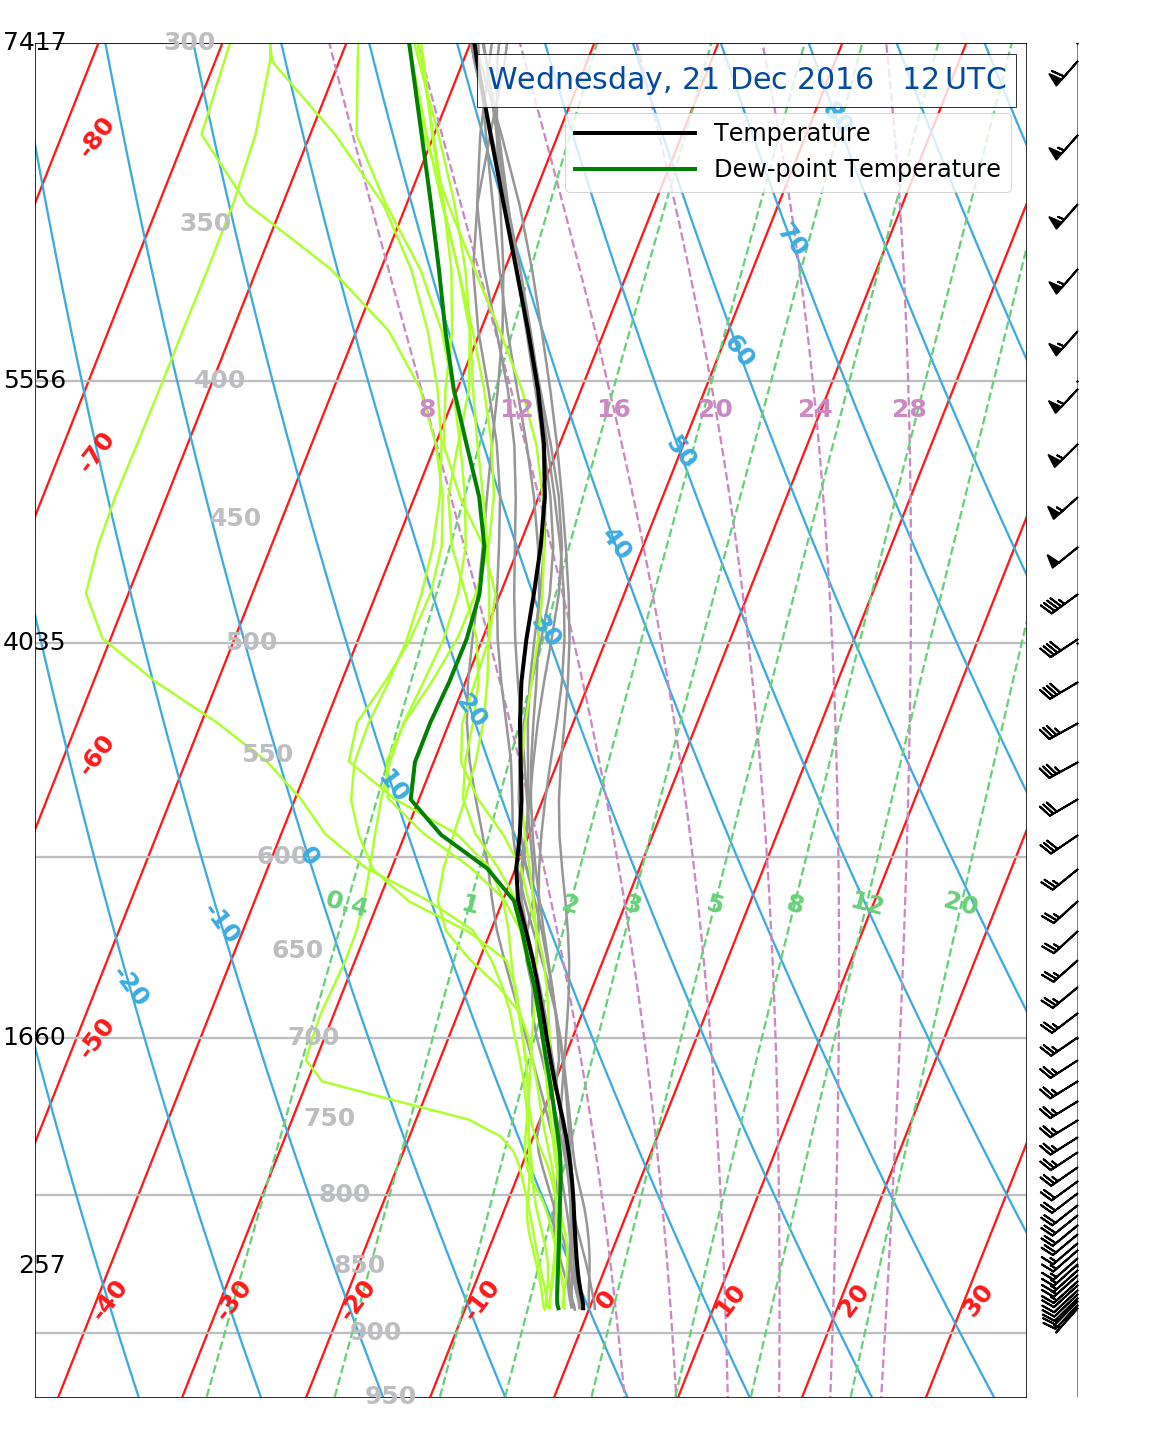
\includegraphics[width=\textwidth]{./fig_Sounding/20161220_36}
		\caption{}\label{fig:meps_sound_20}
	\end{subfigure}
	\begin{subfigure}[b]{0.49\textwidth}
		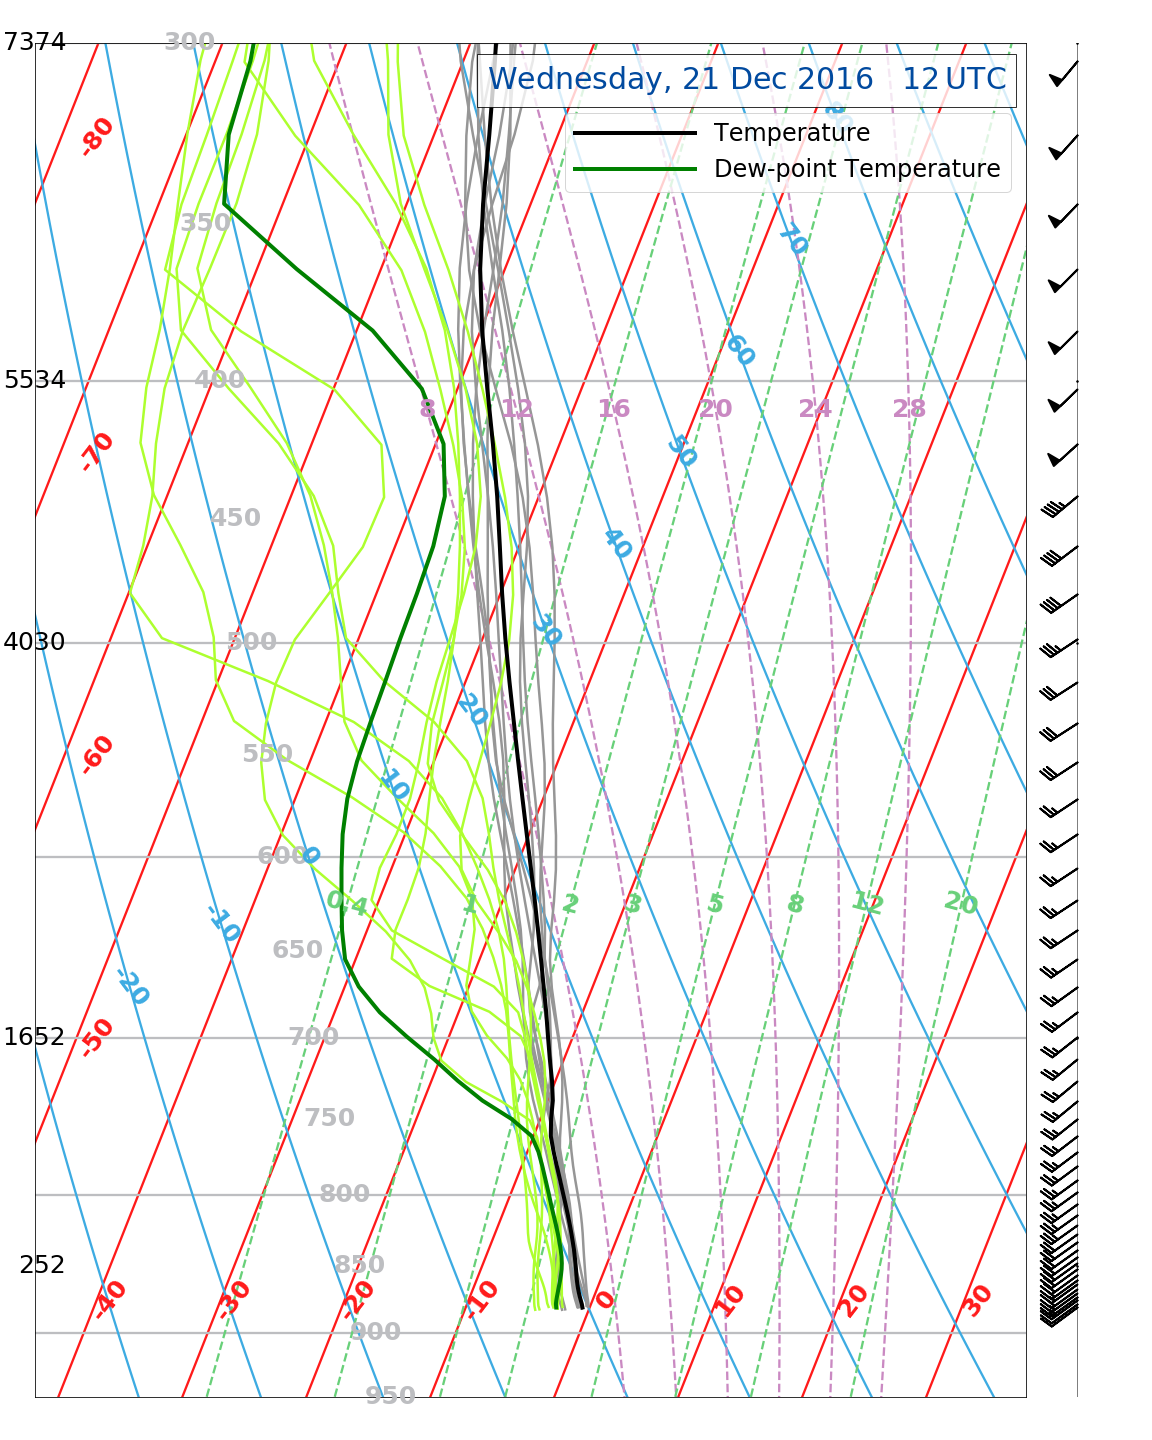
\includegraphics[width=\textwidth]{./fig_Sounding/20161221_12}
		\caption{}\label{fig:meps_sound_21}
	\end{subfigure}
	\caption{Vertical temperature profiles produced with MEPS. \protect{\subref{fig:meps_sound_20}} is initialised: Tuesday, \SI{20}{\dec} \SI{00}{\UTC}. \protect{\subref{fig:meps_sound_21}} is initialised: Wednesday, \SI{21}{\dec} \SI{00}{\UTC}.}
\end{figure}